\documentclass{beamer}

\usetheme[RGB={100, 0, 0}, compress]{Tallahassee}

\usepackage{pgfpages}
% pgfpagesuselayout{resize to}[letterpaper, landscape]
% uncomment usepackage line and next 5 lines to get slides
\pgfpageslogicalpageoptions{1}{border code=\pgfusepath{stroke}}
\pgfpageslogicalpageoptions{2}{border code=\pgfusepath{stroke}}
\pgfpageslogicalpageoptions{3}{border code=\pgfusepath{stroke}}
\pgfpageslogicalpageoptions{4}{border code=\pgfusepath{stroke}}

\usepackage[english]{babel}
\usepackage[T1]{fontenc}
\usepackage{caption}
\usepackage{bibentry}
\usepackage{pifont}
\usepackage{calc}
\usepackage{multicol}
\usepackage{bold-extra}
\usepackage{ulem}
\usepackage{tikz}
\usetikzlibrary{arrows.meta}
\usepackage{setspace}
\usepackage{amsmath}
\usepackage{bbm}
\usepackage{mathtools}
\usepackage{varwidth}
\usepackage{multicol}
\usepackage{algorithm}
\usepackage{algpseudocode}
\usepackage[breakable, theorems, skins]{tcolorbox}
\tikzstyle{block}=[draw opacity=0.7, line width=1.4cm]

\makeatletter
\def\BState{\State\hskip-\ALG@thistlm}
\makeatother

\definecolor{a}{RGB}{175, 0, 0}
\definecolor{b}{RGB}{0, 175, 0}
\definecolor{c}{RGB}{0, 0, 175}
\definecolor{d}{RGB}{175, 0, 175}
\definecolor{e}{RGB}{200, 125, 25}
\definecolor{gray}{RGB}{100, 100, 100}

\definecolor{MyMainColor}{rgb}{0.67,0.00,0.00}
\definecolor{MyRed}{rgb}{0.67,0.00,0.00}
\definecolor{MyDarkBlue}{rgb}{0,0.08,0.55}
\definecolor{MyLightBlue}{rgb}{0,0.08,0.75}
\definecolor{MyGreen}{rgb}{0,0.6,0.25}
\definecolor{MyBlack}{rgb}{0,0,0}
\definecolor{MyBGColor}{rgb}{1.0, 1.0, .8945}

\newcommand{\maincolor}{\textcolor{MyDarkBlue}}
\newcommand{\blacktext}{\textcolor{MyBlack}}
\newcommand{\tantext}{\textcolor{MyBGColor}}
\newcommand{\hi}[1]{\maincolor{\textbf{#1}}}
\newcommand{\tthi}[1]{\maincolor{\textbf{#1}}}
\newcommand{\ex}[1]{\textcolor{red}{\tt #1}}
\newcommand{\win}[1]{\textcolor{Green}{\bf #1}}
\newcommand{\what}[1]{\textcolor{Purple}{\it #1}}
\newcommand{\defeq}{\vcentcolon=}

\newcommand{\hired}[1]{{\usebeamercolor[fg]{alerted text}{\bf #1}}}
\newcommand{\hiblue}[1]{{\usebeamercolor[bg]{block title}{\bf #1}}}
\newcommand{\higreen}[1]{{\usebeamercolor[bg]{block title example}{\bf #1}}}
\newcommand\mymapsto{\mathrel{\ooalign{$\rightarrow$\cr%
			\kern-.15ex\raise.275ex\hbox{\scalebox{1}[0.522]{$\mid$}}\cr}}}

\DeclarePairedDelimiter \norm{\lVert}{\rVert}%
\DeclarePairedDelimiter \abs{\lvert}{\rvert}%

\DeclareRobustCommand{\mybox}[2][gray!20]{%
	\begin{tcolorbox}[   %% Adjust the following parameters at will.
		breakable,
		left=0pt,
		right=0pt,
		top=0pt,
		bottom=0pt,
		colback=#1,
		colframe=#1,
		width=\dimexpr\textwidth\relax, 
		enlarge left by=0mm,
		boxsep=5pt,
		arc=0pt,outer arc=0pt,
		]
		#2
	\end{tcolorbox}
}

\newenvironment{changemargin}[2]{%
  \begin{list}{}{%
    \setlength{\topsep}{0pt}%
    \setlength{\leftmargin}{#1}%
    \setlength{\rightmargin}{#2}%
    \setlength{\listparindent}{\parindent}%
    \setlength{\itemindent}{\parindent}%
    \setlength{\parsep}{\parskip}%
  }%
  \item[]}{\end{list}}

\setbeamertemplate{footline}[frame number]

\begin{document}

\begin{frame}
	\mybox{\centering \Large Toeplitz Inverse Covariance-Based Clustering of
		Multivariate Time Series Data (TICC)}
	\vspace{1.5cm}
	\centering
	{\Large	David Miller} \\ \vspace{.5cm}
	{\Large CIS5930: Social Network Mining} \\
	{\Large Florida State University} \\
	{\Large February 28, 2018}
	
\end{frame}

\section{Introduction}
\subsection{}

%<------------------------------------------------------------------------------
\begin{frame}{Motivation}
	Many things generate large amounts of time series data, most of which is multivariate
	\begin{itemize}
		\item Financial markets
		\item Wearable sensors
		\item Automobiles
	\end{itemize}
	Long term series can be broken down into a sequence of states, each defined by a simple "pattern", where the states can occur multiple times 
	\begin{itemize}
		\item Buy, sell, hold, high volume trading, \dots
		\item Resting, walking, running, \dots
		\item Turning, accelerating, speeding up , \dots
	\end{itemize}
\end{frame}

%<------------------------------------------------------------------------------

\begin{frame}{Motivation: Example}
	\centering
	\begin{figure}
	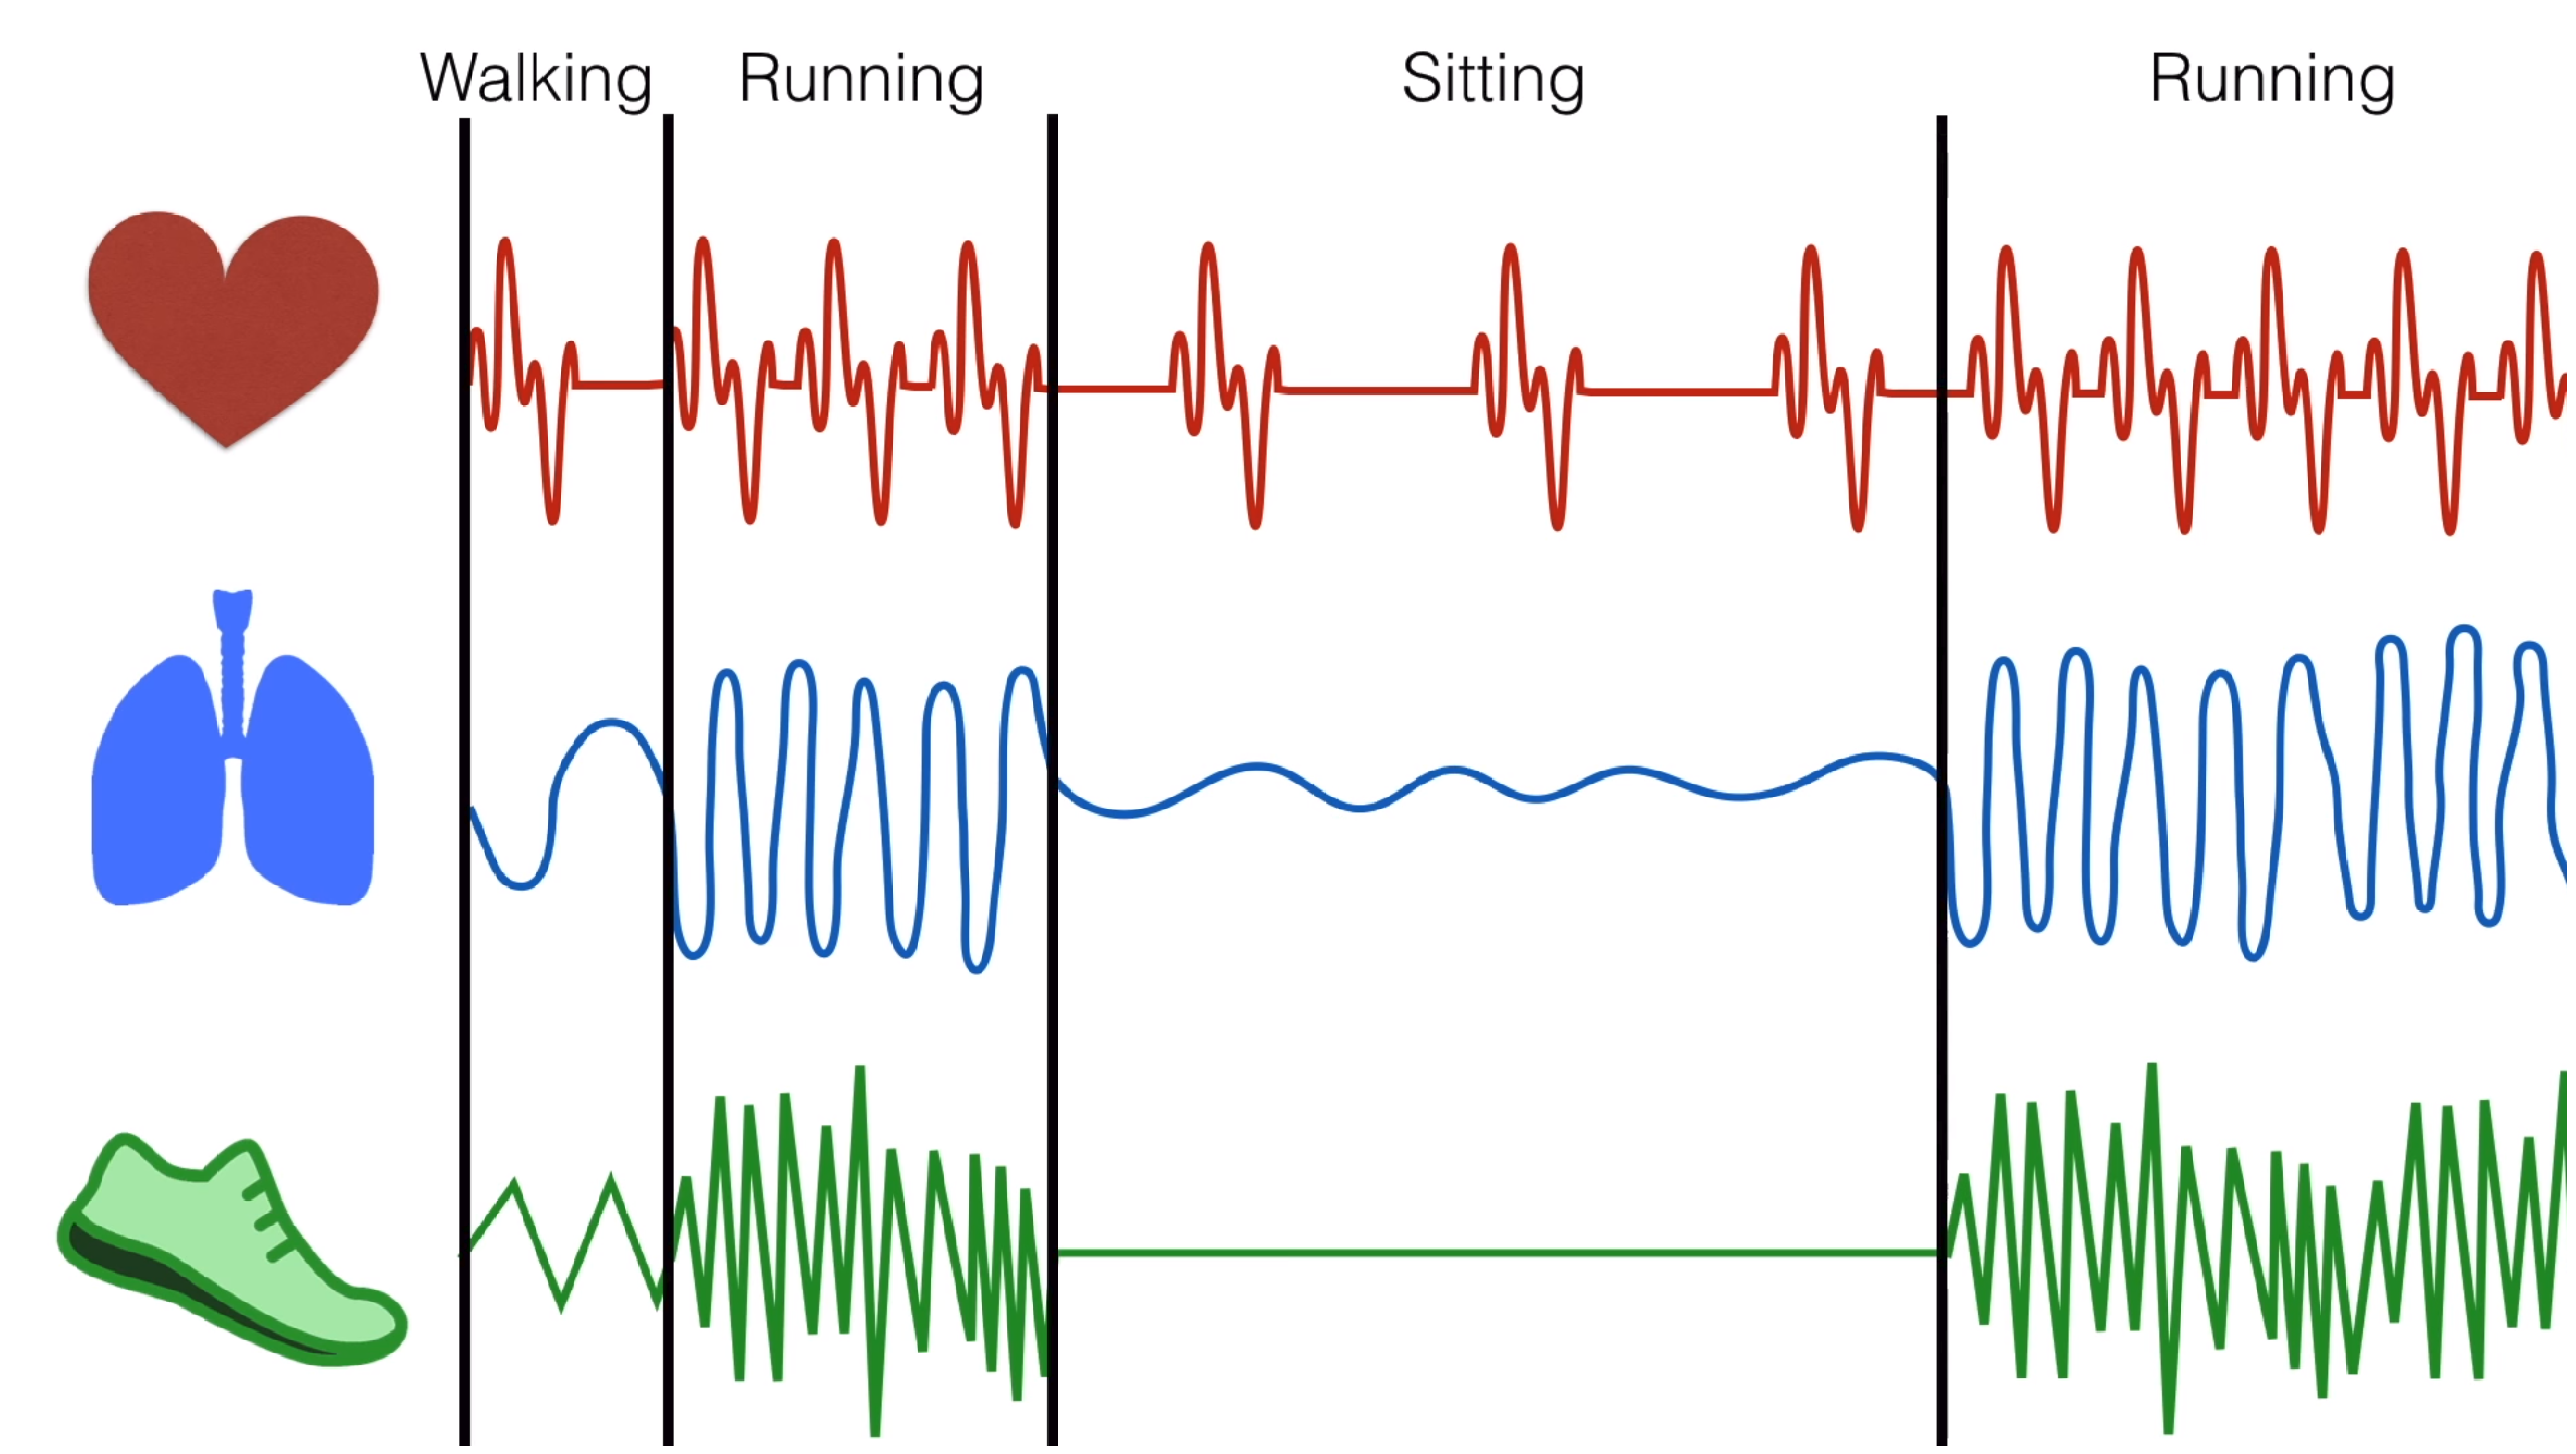
\includegraphics[height=5cm, width=8cm]{fig1.eps}
	\vspace{.25cm}
	\captionsetup{justification=centering, labelformat=empty}
	\caption{Temporal data of heart rate, oxygen usage, and speed with their respective activity (sitting, walking, running) clustering}
	\end{figure}
\end{frame}

%<------------------------------------------------------------------------------

\begin{frame}{Background: Covariance}
	The \textbf{covariance} between two variables is positive when they tend to move in the same direction and negative if they tend to move in opposite directions
	\vspace{.75cm}
	\begin{center}
		\hspace{-1cm}
		\begin{minipage}{.2\textwidth}
			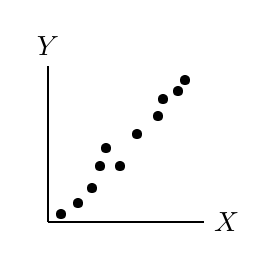
\begin{tikzpicture}[scale=0.33,x=1cm,y=1cm] %[x={10.0pt},y={10.0pt}]
			\draw[thick] (-3,-3)--(3,-3) node [right] {$X$}; % l'axe des abscisses
			\draw[thick] (-3,-3)--(-3,3) node [above] {$Y$};
			\foreach \Point in {(-2.5,-2.75), (-1,-0.89), (2.3,2.41), (.45,.33), 	(2.01,1.97), (1.44, 1.67), (1.23, 1.02), (-1.84,-2.33), (-1.29, -1.76), (-0.75, -.2), (-0.22, -.9) }{
				\node at \Point {\textbullet};}
			\end{tikzpicture} % pic 1
		\end{minipage} \hspace{1.5cm}
		\begin{minipage}{.2\textwidth}
			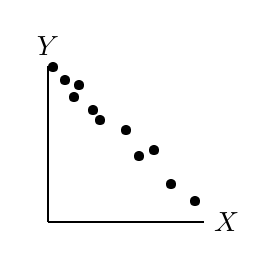
\begin{tikzpicture}[scale=0.33] %[x={10.0pt},y={10.0pt}]
				\draw[thick] (-3,-3)--(3,-3) node [right] {$X$}; % l'axe des abscisses
				\draw[thick] (-3,-3)--(-3,3) node [above] {$Y$};
				\foreach \Point in {(-2.8, 2.9), (0,.5), (1.75, -1.6), (2.69, -2.23), 
				(-2, 1.76), (-2.33, 2.4), (-1.78, 2.21), (-1.25, 1.25), (-1,.86),
				(.5,-.5), (1.11, -.28)}{
					\node at \Point {\textbullet};}
			\end{tikzpicture} % pic 2
		\end{minipage} \hspace{1.5cm}
		\begin{minipage}{.2\textwidth}
			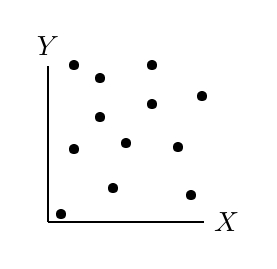
\begin{tikzpicture}[scale=0.33] %[x={10.0pt},y={10.0pt}]
				\draw[thick] (-3,-3)--(3,-3) node [right] {$X$}; % l'axe des abscisses
				\draw[thick] (-3,-3)--(-3,3) node [above] {$Y$};
				\foreach \Point in {(-2.5,-2.75), (-1,1), (-2,3), (-1,2.5), (1,3), 
					(2.5, -2), (0,0), (1, 1.5), (-2, -.25), (-.5, -1.75), 
					(2.95, 1.8), (2, -.175)}{
					\node at \Point {\textbullet};}
			\end{tikzpicture} % pic 3
		\end{minipage}
		\end{center}
		\hspace{.1cm} Positive covariance \hspace{.6cm} Negative covariance \hspace{.6cm} Zero covariance
\end{frame}

%<------------------------------------------------------------------------------

\begin{frame}{Background: Markov Random Field (MRF)}
	A \textbf{Markov Random Field} is an undirected graph $G = (V,E)$ such that $V$ are random variables and
	\begin{itemize}
		\item If $(v_i,v_j) \not\in E$ then random variables $i$ and $j$ are conditionally independent given $V \setminus \{v_i,v_j\}$
		\item Random variable $i$ is conditionally independent of random variable $j$ if $d(v_i,v_j) > 1$ given all $v_j$ s.t. $d(v_i,v_j) = 1$
		\item $A = \{v_1, \dots, v_n\}$ is conditionally independent of $B = \{v_1, \dots, v_m\}$ given some set $S$ such that every path from a node in $A$ to a node in $B$ passes through $S$ 
	\end{itemize}
\end{frame}

%<------------------------------------------------------------------------------

\begin{frame}{Background: Markov Random Field (MRF)}
\begin{minipage}{.475\textwidth}
	$A$ depends on $E$ \\
	$B$ depends on $D$ and $E$ \\
	$C$ depends on $D$ and $F$ \\
	$D$ depends on $B, C, E,$ and $F$ \\
	$E$ depends on $A, B,$ and $D$ \\
	$F$ depends on $C$ and $D$ \\ 
\end{minipage}% 
\hspace{.05cm}
\begin{minipage}{.475\textwidth}
\begin{center}
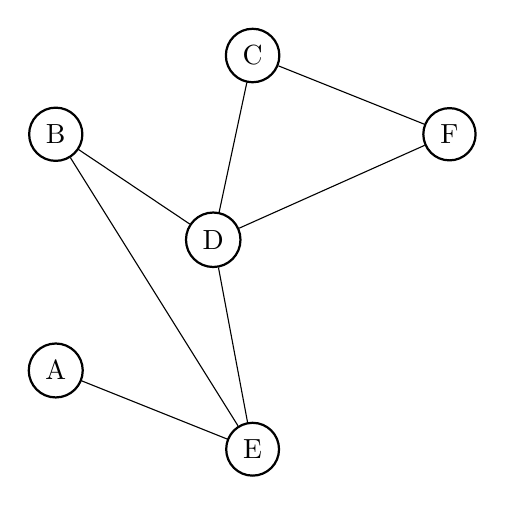
\begin{tikzpicture}
\node[shape=circle,draw=black,thick] (A) at (0,0) {A};
\node[shape=circle,draw=black,thick] (B) at (0,3) {B};
\node[shape=circle,draw=black,thick] (C) at (2.5,4) {C};
\node[shape=circle,draw=black,thick] (D) at (2,1.66) {D};
\node[shape=circle,draw=black,thick] (E) at (2.5,-1) {E};
\node[shape=circle,draw=black,thick] (F) at (5,3) {F} ;

\path (B) edge (E);
\path (B) edge (D);
\path (D) edge (C);
\path (A) edge (E);
\path (D) edge (E);
\path (D) edge (F);
\path (C) edge (F);  
\end{tikzpicture}
\end{center}
\end{minipage}
\end{frame}

%<------------------------------------------------------------------------------

\begin{frame}{Background: Toeplitz Matrix}
	A \textbf{Toeplitz Matrix} is a matrix such that each descending diagonal from left to right is constant. Let A be a $n \times n$ Toeplitz matrix, then $A$ takes on the form
	\begin{align*}
		A =
		\begin{bmatrix}
			a_0     & a_{-1} & a_{-2}  & \dots  & \dots  & a_{-(n-1)} \\
			a_1     & a_0    & a_{-1}  & \ddots &        & \vdots     \\
			a_2     & a_1    & \ddots  & \ddots & \ddots & \vdots     \\
			\vdots  & \ddots & \ddots  & \ddots & a_{-1} & a_{-2}     \\
			\vdots  &        & \ddots  & a_1    & a_0    & a_{-1}     \\
			a_{n-1} & \dots  & \dots   & a_2    & a_1    & a_0
		\end{bmatrix}
	\end{align*}
	where the $i,j$ element $A_{i,j} = A_{i+1,j+1} = a_{i-j}$
\end{frame}

%<------------------------------------------------------------------------------

\begin{frame}{Background: Inverse Covariance Matrix}
	The \textbf{inverse covariance matrix} essentially models the dependency, or relation, of variables with their neighbors. Take for example the multiple mass-spring problem
	\begin{align*} 
		m\ddot{x_i} = -k(x_i-x_{i-1}) - k(x_{i+1}-x_i) + w_i \hspace{.75cm} \\
		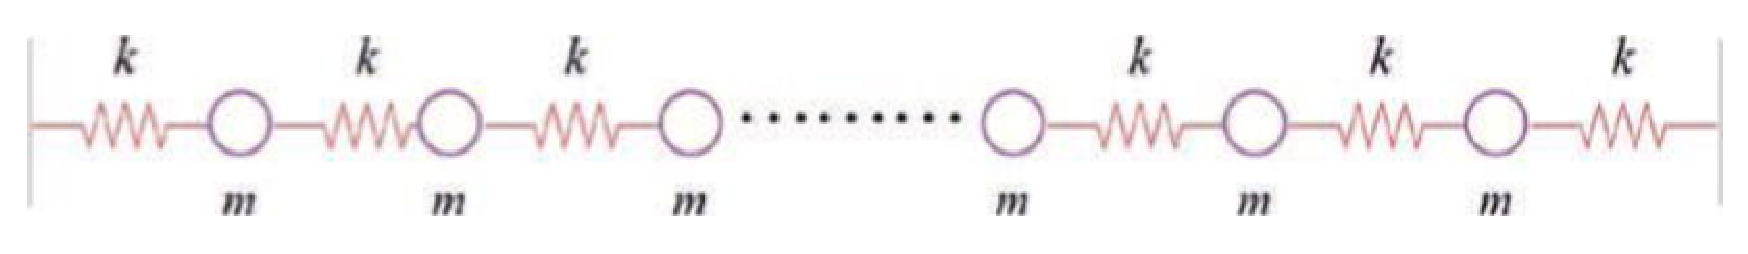
\includegraphics[height=1cm,width=8cm]{fig9.eps}
	\end{align*}
	where $x_i$ is displacement of $m_i$ and $w_i$ is external force acting on $m_1$. This can be written in matrix form
	\begin{align*}
		m
		\begin{bmatrix}
			\ddot{x}_1 \\
			\ddot{x_2} \\
			\vdots \\
			\ddot{x_n}
		\end{bmatrix} = k
		\underbrace{
		\begin{bmatrix}
			-2 & 1 & 0 & \dots & 0 \\
			1 & -2 & 1 & 0 & \dots \\
			0 & \ddots & \ddots & \ddots & \\
			0 & \dots & \dots & 1 & -2  
		\end{bmatrix}
		}_{\text{Inverse covariance matrix}}
		\begin{bmatrix}
			x_1 \\
			x_2 \\
			\vdots \\
			x_n
		\end{bmatrix} +
		\begin{bmatrix}
			w_1 \\
			w_2 \\
			\vdots \\
			w_n
		\end{bmatrix}
	\end{align*}
\end{frame}

%<------------------------------------------------------------------------------

\section{Problem Setup}
\subsection{}

\begin{frame}{Problem Statement}
	Given a time series of $T$ sequential observations
	\begin{align*} 
	x_{orig} =
	\begin{bmatrix}
		|   &   |   &   |   &        &  |  \\
		x_1 &  x_2  &  x_3  &  \dots & x_T \\
		|   &   |   &   |   &        &  |  
	\end{bmatrix}
	\end{align*}
	where $x_i \in \mathbb{R}^n$ is the $i$-th multivariate observation, \textbf{the goal is to cluster these $\boldsymbol{T}$ observations into $\boldsymbol{K}$ clusters}. The dimension $n$ is typically the number of sensors of the data.
\end{frame}

%<------------------------------------------------------------------------------

\begin{frame}{Problem Statement}
	Instead of clustering each observation $x_i$ in isolation, each point is treated  in context of its previous $w - 1$ predecessors, where $w \ll T$. We then have
	\begin{align*}
		X_t \defeq
		\begin{bmatrix}
		x_{t-w+1} \\
		x_{t-w+2} \\
		\vdots \\
		x_{t-1} \\
		x_{t}
		\end{bmatrix}
	\end{align*}
	where $X_t \in \mathbb{R}^{nw}$. Let the sequence $X_1, \dots, X_T$ be referred to as $X$. Now \textbf{the goal is to cluster these subsequences $\boldsymbol{X_1}$, ..., $\boldsymbol{X_T}$}. The mapping $f:x_{orig} \rightarrow X$ is a bijection.
\end{frame}

%<------------------------------------------------------------------------------

\begin{frame}{Toeplitz Inverse Covariance-Based Clustering (TICC)}
	Each cluster is defined by a Gaussian inverse covariance $\Theta_i \in \mathbb{R}^{nw \times nw}$.  These inverse covariances show the conditional independency structure between the variables that define a MRF encoding the structural representation of each cluster \cite{26}. \\
	\vspace{.5cm}
	The objective is to solve for these $K$ inverse covariances $\boldsymbol{\Theta} = \{\Theta_1, \dots, \Theta_K\}$ and assignment sets $\boldsymbol{P} = \{P_1, \dots, P_k\}$ via the optimization problem, or the TICC problem.
\end{frame}

%<------------------------------------------------------------------------------

\begin{frame}{Toeplitz Inverse Covariance-Based Clustering (TICC)}
	The TICC problem is
	\begin{align*}
		\footnotesize
		\arg\min\limits_{\boldsymbol{\Theta} \in \mathcal{T}, \boldsymbol{P}} \sum\limits_{i=1}^K\bigg[ \overbrace{\norm{\lambda \circ \Theta_i}_1}^{\text{sparsity}} + \sum\limits_{X_t \in P_i} \bigg( \overbrace{-\ell\ell(X_t, \Theta_i)}^{\text{log likelihood}} + \overbrace{\beta\mathbbm{1}\{X_{t-1} \not\in P_i \}}^{\text{temporal consistency}} \bigg) \bigg]
		\tag{1}
	\end{align*}
	where $\mathcal{T}$ is the set of symmetric block Toeplitz $nw \times nw$ matrices, $\norm{\lambda \circ \Theta_i}_1$ is an $\ell_1$-norm penalty to incentivize a sparse inverse covariance, and $\mathbbm{1}\{X_t-1 \not\in P_i\}$ is an indicator function checking whether neighboring points are assigned to the same cluster. Additionally, $\ell\ell(X_t, \Theta_i)$ is the log likelihood that $X_i$ came from cluster $i$,
	\begin{align*}
		\ell\ell(X_t, \Theta_i) = -\frac{1}{2}(X_t - \mu_i)^T \Theta_i(X_t - \mu_i) + \frac{1}{2}\log\det\Theta_i - \frac{n}{2}\log(2\pi) 
	\end{align*}
	where $\mu_i$ is the empirical mean of cluster $i$.
\end{frame}

%<------------------------------------------------------------------------------

\begin{frame}{Regularization Parameters}
	The TICC optimization problem has two regularization parameters
	\begin{itemize}
		\item $\beta$: Smoothness penalty that encourages adjacent subsequences to be assigned to the same cluster.
		\item $\lambda$: Determines the sparsity of level in the MRFs characterizing each cluster. Although it is a $nw \times nw$ matrix, all its values are typically set to a single value to reduce the search space to one parameter. 
	\end{itemize}
	Parameters can be manually set if given prior knowledge or determined through some method, such as Bayesian information criterion (BIC).
\end{frame}

%<------------------------------------------------------------------------------

\begin{frame}{A Note on the Inverse Covariances}
	The inverse covariances $\Theta_i$'s are constrained to be block Toeplitz, thus can be expressed in the form
	\begin{align*}
		\Theta_i = 
		\begin{bmatrix}
		A^{(0)} & (A^{(1)})^T & (A^{(2)})^T & \dots   & \dots       & (A^{(w-1)})^T \\
		A^{(1)} & A^{(0)}     & (A^{(1)})^T & \ddots  &             & \vdots        \\
		A^{(2)} & A^{(1)}     & \ddots		& \ddots  & \ddots      & \vdots        \\
		\vdots  & \ddots      & \ddots      & \ddots  & (A^{(1)})^T & (A^{(2)})^T   \\
		\vdots  &             & \ddots      & A^{(1)} & A^{(0)}     & (A^{(1)})^T   \\
		A^{(w-1)} & \ddots  & \ddots      & A^{(2)} & A^{(1)}     & A^{(0)}
		\end{bmatrix}
	\end{align*} 
	where $A^{(0)}, A^{(1)}, \dots, A^{(w-1)} \in \mathbb{R}^{n \times n}$.
\end{frame}

%<------------------------------------------------------------------------------

\begin{frame}{A Note on the Inverse Covariances}
	Diagonal blocks $A^{(0)}$ represent the intra-time partial correlations. \\
	\vspace{.5cm}
	Off diagonal block $A^{(n)}_{jk} \in \Theta_i$ shows how sensor $i$ at some time $t$ is correlated to sensor $j$ at time $t+n$. \\
	\vspace{.5cm}
	The block Toeplitz structure of the inverse covariance means that we are making a time-invariance assumption over the length-$w$ window. That is, if edges between layer $m$ and layer $n$, where $m < n$, also exists in layers $n + (n - m), n + 2(n - m), \dots$.  
\end{frame}

%<------------------------------------------------------------------------------

\begin{frame}{Problem: Example}
	\begin{figure}
		\centering
		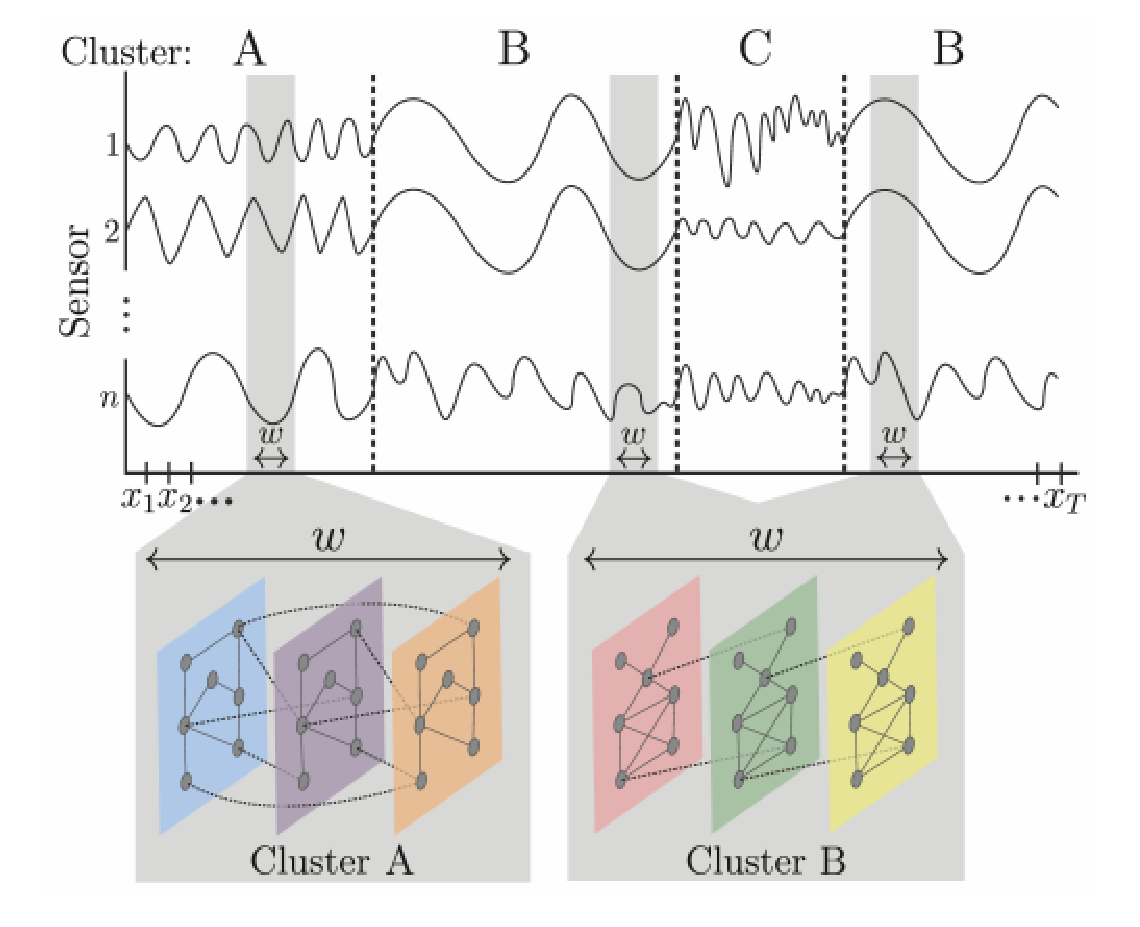
\includegraphics[width=7cm]{fig3.eps}
	\end{figure}
	\centering
	Edges across layers within the same time window are time invariant and need not be a distance of 1 apart.
\end{frame}

%<------------------------------------------------------------------------------

\section{Alternating Minimization}
\subsection{}

\begin{frame}{Expectation-Maximization (EM)}
	The TICC problem is a mixed combinatorial and continuous optimization problem. The cluster assignments $P$ and inverse covariences $\Theta$ coupled together make the problem highly non-convex. As such, there is no tractable way to solve for the globally optimal solution. \\
	\vspace{.5cm}
	A variation of the EM algorithm is used to alternate between assigning points to clusters and then updating the cluster parameters.
\end{frame}

%<------------------------------------------------------------------------------

\begin{frame}{Assigning Points to Clusters}
	Points are assigned to clusters by fixing $\Theta$ and solving the following optimization problem for $\boldsymbol{P} = \{P_1, \dots, P_K\}$
	\begin{align*}
		\text{minimize}\sum\limits_{i=1}^K\sum\limits_{X_t \in P_i} -\ell\ell(X_t, \Theta_i) + \beta\mathbbm{1}\{X_{t-1} \not\in P_i\} \tag{2}
	\end{align*}
	This problem assigns each $X_t$ subsequence to one of the $K$ clusters to jointly maximize the log likelihood and the temporal consistency, with the tradeoff between the two objectives being regulated by $\beta$. \\
	\vspace{.5cm}
	If $\beta = 0$ then $X_1, \dots, X_t$ can be assigned independently since there is no penalty to encourage neighboring subsequences to belong to the same cluster. As $\beta \rightarrow \infty$, switching penalty becomes so large that all $X_t$ are grouped into just one cluster.
\end{frame}

%<------------------------------------------------------------------------------

\begin{frame}{Toeplitz Graphical Lasso}
	Given $\boldsymbol{P}$ from EM, the cluster parameters $\Theta_1, \dots, \Theta_K$ are updated by solving the TICC problem while holding $\boldsymbol{P}$ constant. After some recasting the cluster parameters can be solved in parallel via
	\begin{align*}
		\text{minimize} \hspace{1cm} & -\log\det\Theta_i + \text{tr}(S_i\Theta_i) + \frac{1}{\abs{P_i}}\norm{\lambda \circ \Theta_i}_1 \tag{3} \\
		\text{subject to} \hspace{1cm} & \Theta_i \in \mathcal{T} \tag{3.1}
	\end{align*}
	where $\abs{P_i}$ is the number of points assigned to cluster $i$, and $S_i$ is the empirical covariance of these points. This optimization problem is the Toeplitz graphical lasso. 
\end{frame}

%<------------------------------------------------------------------------------

\section{Algorithm}
\subsection{}

\begin{frame}{Cluster Assignment}
	\begin{minipage}{.4\textwidth}
	Given $K$ potential cluster assignments of the $T$ points, this combinatorial
	optimization problem has $K^T$ possible assignments of points to clusters. Cluster assignment are solved in $\mathcal{O}(KT)$ using  dynamic programming approach that is equivalent to finding the minimum cost Viterbi path. 
	\end{minipage}%
	\hspace{.1cm}
	\begin{minipage}{.575\textwidth}
		\begin{figure}
			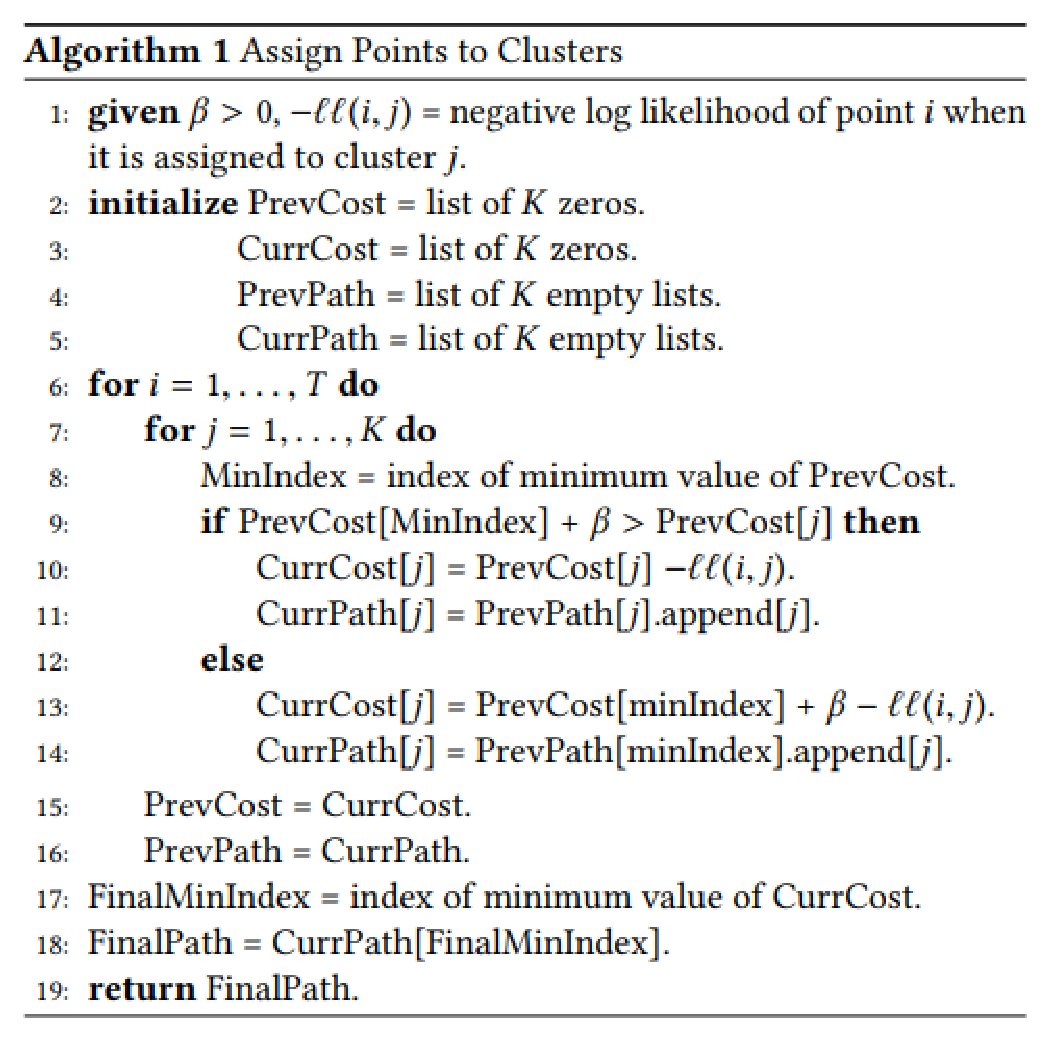
\includegraphics[height=6.5cm, width=6.25cm]{fig6.eps}
		\end{figure}
	\end{minipage}
\end{frame}

%<------------------------------------------------------------------------------

\begin{frame}{Cluster Assignment}
	\begin{figure}
		\centering
		\includegraphics[width=7.5cm]{fig7.eps}
		\caption*{\centering Problem 3 is equivalent to finding the minimum cost path from timestamp 1 to $T$, where the node cost is the negative log likelihood of that point being assigned to a cluster, and the edge cost is $\beta$ whenever the cluster assignment switches.}
	\end{figure}
\end{frame}

%<------------------------------------------------------------------------------

\begin{frame}{Solving the Toeplitz Graphical Lasso}
	Alternating direction method of multipliers (ADMM) and augmented Lagrangian are used to efficiently solve the Toeplitz graphical lasso. First problem 3 is recast into ADMM form
	\begin{align*}
		\text{minimize} \hspace{1cm} & -\log\det\Theta_i + \text{tr}(S_i\Theta_i) + \frac{1}{\abs{P_i}}\norm{\lambda \circ Z}_1 \\
		\text{subject to} \hspace{1cm} & \Theta_i = Z, Z \in \mathcal{T} 
	\end{align*}
	The augmented Lagrangian can then be expressed as
	\begin{align*}
		\mathcal{L}_\rho(\Theta, Z, U) = -\log\det(\Theta) + \textbf{Tr}(S\Theta) + \norm{\lambda \circ Z}_1 + \frac{\rho}{2}\norm{\Theta - Z + U}_F^2
	\end{align*}
	where $\rho > 0$ is the ADMM penalty parameter and $U \in \mathbb{R}^{nw \times nw}$ is the scalable dual variable. 
\end{frame} 

%<------------------------------------------------------------------------------

\begin{frame}{The TICC Algorithm}
	The algorithm consists of the following three steps repeated until convergence
	\begin{align*}
		(a) \hspace{.5cm} & \Theta^{k+1} \defeq \arg\min\limits_{\Theta} \mathcal{L}_\rho(\Theta, Z^k, U^k) \\
		(b) \hspace{.5cm} & Z^{k+1} \defeq \arg\min\limits_{Z \in \mathcal{T}} \mathcal{L}_\rho(	\Theta^{k+1}, Z, U^k) \\
		(c) \hspace{.5cm} & 	U^{k+1} \defeq U^k + (\Theta^{k+1}- Z^{k+1})
	\end{align*}
	where $k$ is the iteration number. The stopping criterion is for the algorithm is Residual$(\Theta, Z, U) < \epsilon$ for some arbitrarily small $\epsilon$. Solving (b) requires solving $(w-1)n^2 + \frac{n(n-1)}{2}$ subproblems, which can all be done in parallel.  Problem (a) has known analytic solution, see \cite{paper} for solution to (b). 
\end{frame}

%<------------------------------------------------------------------------------

\begin{frame}{The TICC Algorithm}
	\begin{figure}
		\centering
		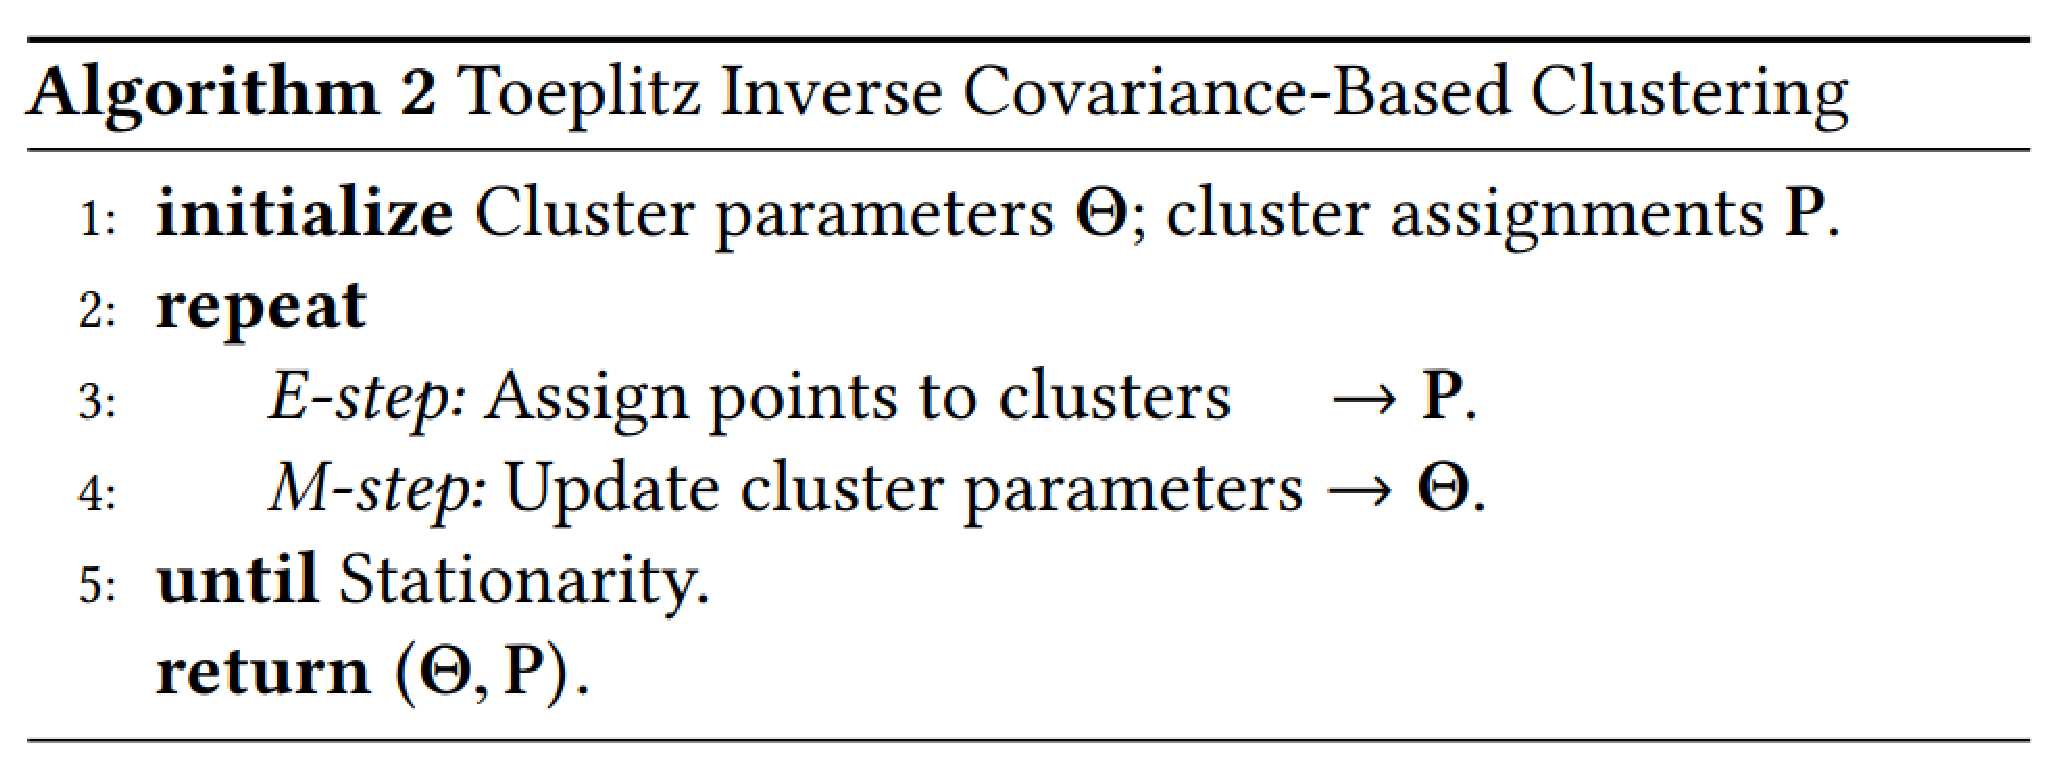
\includegraphics[width=10cm]{fig8.eps} \\ 
		\vspace{.25cm}
		\caption*{\centering The TICC algorithm can be broken down into two key parts: $i)$ solving the cluster assignment problem and then $ii)$ solving for cluster inverse covariances until convergence.}
	\end{figure}
\end{frame}

%<------------------------------------------------------------------------------

\section{Results and Conclusions}
\subsection{}

\begin{frame}{Implementation}
	A custom Python solver is built to run the TICC algorithm.
	\begin{itemize}
		\item Input: Original multivariate time series and problem parameters
		\item Output: The clustering assignments of each point in the time series, along with the structural MRF representation of each cluster
	\end{itemize}
	\vspace{.5cm}
	TICC is tested on several synthetic examples because there are "ground truth" clusters to evaluate the accuracy of the method. 
\end{frame}

%<------------------------------------------------------------------------------

\begin{frame}{Generating Datasets}
	Synthetic multivariate data in $\mathbb{R}^5$ is randomly generated. Each of the $K$ clusters has a mean $\vec{0}$ so that the clustering result is based entirely on the structure of the data. For each cluster, random ground truth Toeplitz iverse covariance is generated as 
	\begin{itemize}
		\item Set $A^{(0)}, \dots, A^{(4)}$ equal to adjacency matrices of 5 independent Erd\H{o}s-R\'{e}nyi where each edge has a 20\% of \\ being selected
		\item For every selected edge in $A^{(m)}$ set $A^{(m)}_{jk} = v_{jk,m}$ a random weight centered at 0
		\item Construct a $5w \times 5w$ block Toeplitz matrix $G$, where window size $w = 5$, using the blocks $A^{(0)}, \dots, A^{(4)}$
		\item Let $c$ be the smallest eigenvalue of $G$ and set $\Theta_i = G + 0.1 + \abs{c}I$. This ensures that $\Theta_i$ is invertible
	\end{itemize}
\end{frame}

%<------------------------------------------------------------------------------

\begin{frame}{Generating Datasets}
	The overall time series is then generated by constructing a temporal sequence of cluster segments (for example, the sequence "1,2,1" with 200 samples in each of the segments,  coming from two inverse covariances $\Theta_1$ and $\Theta_2$).\\
	\vspace{.5cm}
	Experiments are run on four different temporal sequences: "1,2,1", "1,2,3,2,1", "1,2,3,4,1,2,3,4", "1,2,2,1,3,3,3,1". Each segment in each of the examples has 100$K$ observations in $\mathbb{R}^5$, where $K$ is the
	number of clusters in that experiment (2, 3, 4, and 3, respectively). $K$ is fixed to be the "true" number of clusters for both TICC and the baseline methods.
\end{frame}

%<------------------------------------------------------------------------------

\begin{frame}{Baseline Methods}
	\begin{itemize}
		\item TICC, $\beta$ = 0: TICC and TICC without temporal consistency constraint
		\item GMM: Clustering using a Gaussian Mixture Model
		\item EEV: Regularized GMM with shape and volume constraints on the Gaussian covariance matrix
		\item DTW, GAK: Dynamic time warping-based clustering using a global alignment kernel
		\item DTW, Euclidean: DTW using a Euclidean distance metric
		\item Nerual Gas: Artificial neural network clustering method based on self-organizing maps
		\item K-means: Standard K-means clustering algorithm using Euclidean distance
	\end{itemize}
\end{frame}

%<-------------------------------------------------------------------------------

\begin{frame}{Results}
	\begin{center}
	\begin{tabular}{c||c|c|c|c}
		\hline
		 Method & 1,2,1 & 1,2,3,2,1 & 1,2,3,4,1,2,3,4 & 1,2,2,1,3,3,3,1 \\ \hline\hline
		 \textbf{TICC} & \textbf{0.92} & \textbf{0.90} & \textbf{0.98} & \textbf{0.98} \\ \hline
		 TICC, $\beta=0$ & 0.88 & 0.89 & 0.86 & 0.89 \\ \hline
		 GMM & 0.68 & 0.55 & 0.83 & 0.62 \\ \hline
		 EEV & 0.59 & 0.66 & 0.37 & 0.88 \\ \hline
		 DTW, GAK & 0.64 & 0.33 & 0.26 & 0.27 \\ \hline 
		 DTW, Euclid & 0.50 & 0.24 & 0.17 & 0.25 \\ \hline
		 Neural Gas & 0.52 & 0.35 & 0.27 & 0.34 \\ \hline
		 K-means & 0.59 & 0.34 & 0.24 & 0.34 \\ \hline
	\end{tabular}
	\\
	\vspace{.25cm}
	Macro-$F_1$ scores of clustering accuracy for four different temporal sequences.
	\end{center}
\end{frame}

%<-------------------------------------------------------------------------------

\begin{frame}{Results}
	\begin{figure}
		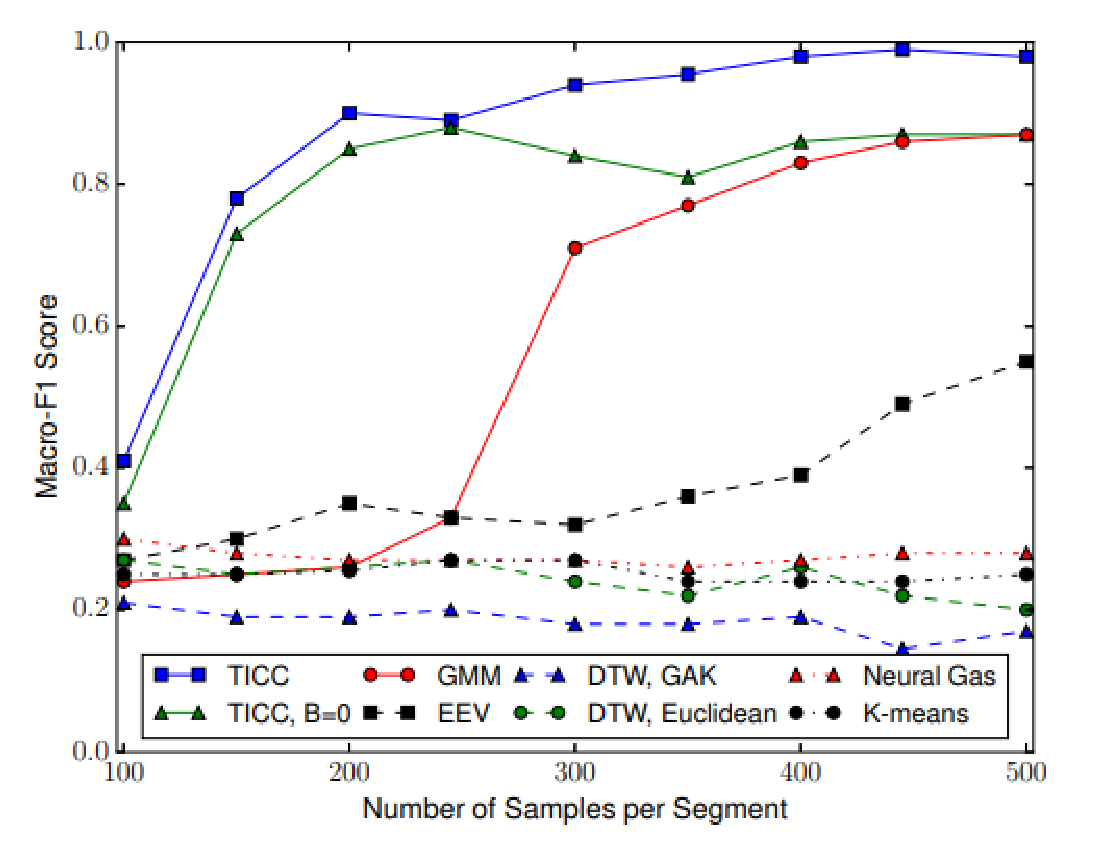
\includegraphics[width=7.25cm]{fig4.eps}
		\caption*{\centering Clustering accuracy macro-$F_1$ score vs number of samples. TICC needs significantly fewer samples than other methods to achieve similar performance.}
	\end{figure}
\end{frame}

%<-------------------------------------------------------------------------------

\begin{frame}{Case Study}
	TICC is applied to a large dataset from a one-hour driving session where 7 sensors are observed every 0.1 seconds
	\begin{multicols}{2}
		\begin{itemize}
			\item Brake Pedal Position
			\item Forward(X)-Acceleration
			\item Lateral(Y)-Acceleration
			\item Steering Wheel Angle
		\end{itemize}%
		\columnbreak
		\begin{itemize}
			\item Vehicle Velocity
			\item Engine RPM
			\item Gas Pedal Position
		\end{itemize}
	\end{multicols}
	TICC is applied with $w = 10$ (1 second window size). Number of clusters picked using BIC, then discovered that $K = 5$ is optimal.
\end{frame}

%<-------------------------------------------------------------------------------

\begin{frame}{Case Study}
	\begin{center}
		\footnotesize
		\begin{tabular}{c||c|c|c|c|c|c|c}
			 & Brake & X-Acc & Y-Acc & SW Angle & Vel & RPM & Gas \\ \hline\hline
			 Slow Down & 25.64 & 0 & 0 & 0 & 27.16 & 0 & 0 \\ \hline
			 Turning & 0 &  4.24 &  66.01 &  17.56 &  0 &  5.13 & 135.1 \\ \hline
			 Speed Up &  0 &  0 &  0 &  0 & 16.00 &  0 &  4.50 \\ \hline
			 Drive Straight &  0  & 0 &  0 &  0 & 32.2 &  0 &  26.8 \\ \hline
			 Curvy Road &  4.52 &  0 &  4.81 &  0 &  0 &  0 &  94.8 \\ \hline
		\end{tabular}\\
		\vspace{.5cm}
		{\normalsize Betweenness centrality for each sensor in each of the five clusters. This score can be used as a proxy to show the "importance" of each sensor is and how it directly affects other sensor values} 
	\end{center}
\end{frame}

%<-------------------------------------------------------------------------------

\begin{frame}{Case Study}
	\begin{figure}
		\centering
		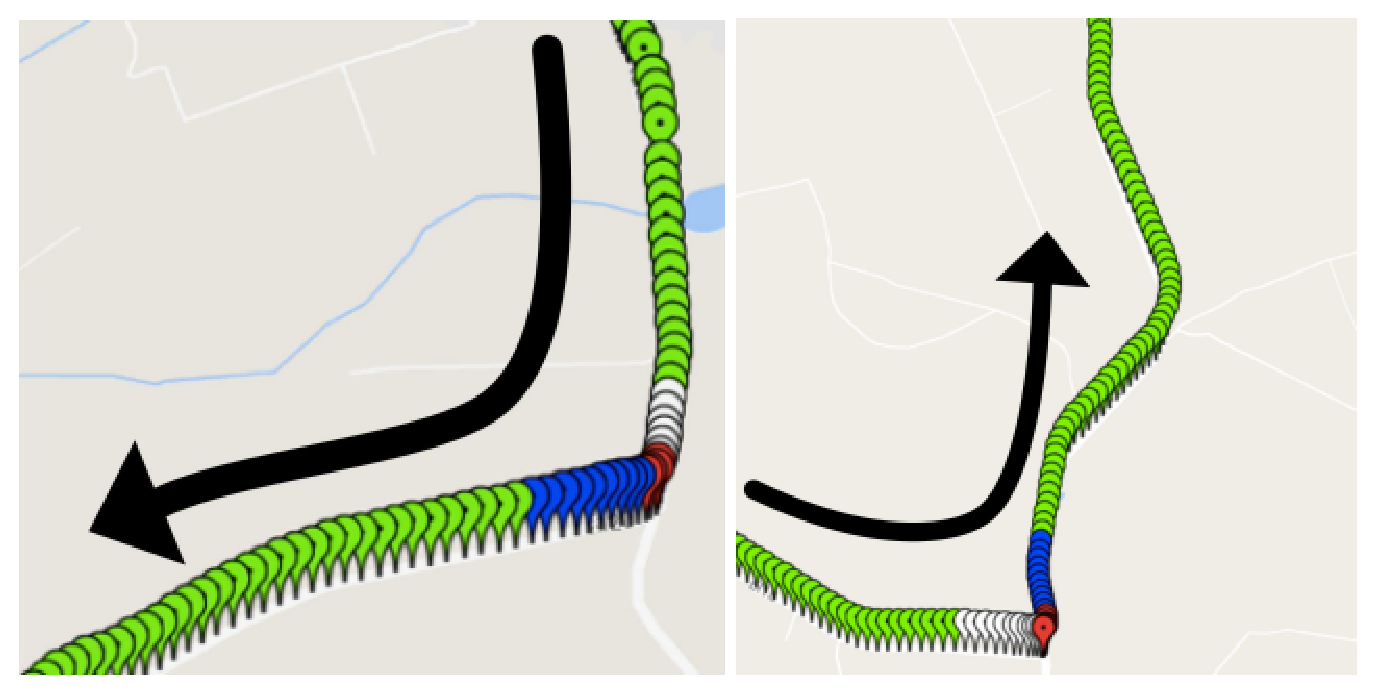
\includegraphics[width=9cm, height=3.67cm]{fig5.eps}
		\caption*{\centering Pins represent cluster assingments. The color clusters are  Green = Going Straight  White = Slowing Down, Red = Turning, Blue = Speeding Up.}
	\end{figure}
\end{frame}

%<-------------------------------------------------------------------------------

\begin{frame}{References}
\begin{thebibliography}{acm}
	\bibitem{paper}
	David Hallac, Sagar Vare, Stephen Boyd, Jure Leskovec. \textit{Toeplitz Inverse Covariance-Based Clustering of Multivariate Time Series Data.} KDD’17, August 13–17, 2017, Halifax, NS, Canada
	\bibitem{26}
	D. Koller and N. Friedman. \textit{Probabilistic Graphical Models: Principles and Techniques.} MIT press, 2009.
\end{thebibliography}
\end{frame}





\end{document}

